\documentclass{article}
\usepackage{graphicx}
\usepackage[margin=1.5cm]{geometry}
\usepackage{amsmath}

\begin{document}
\twocolumn

\title{Monday Warm Up: Unit 4, Reactance, RL circuits, RLC circuits}
\author{Prof. Jordan C. Hanson}

\maketitle

\section{Memory Bank}

\begin{itemize}
\item $\tau = RC$ ... The time constant of an RC circuit.
\item $f_0 = \frac{1}{2\pi\sqrt{LC}}$ ... RLC circuit resonance frequency.
\item $i(t) = \frac{\epsilon}{R}\left(1 - \exp(-t/\tau) \right)$ ... Charging RL circuit.
\item $i(t) = \frac{\epsilon}{R}\exp(-t/\tau)$ ... Discharging RL circuit.
\item $\tau = L/R$ ... Time constant of an RL circuit.
\item $V_{\rm rms} = I_{\rm rms} Z_{\rm tot}$ ... Ohm's Law for AC circuits.
\item $P_{\rm ave} = I_{\rm ave} V_{\rm ave}\cos\phi$ ... Average power in series RLC circuit.
\item $X_{\rm C} = 1/(2\pi f C)$ ... Reactance of a capacitor.
\item $X_{\rm L} = 2\pi f L$ ... Reactance of an inductor.
\item $Z_{\rm tot} = \sqrt{R^2 + (X_{\rm L} - X_{\rm C})^2}$ ... The total impedance of an RLC series circuit.
\item $\cos\phi = R/Z_{\rm tot}$ ... Power factor of an RLC series circuit.
\end{itemize}

\section{RL Circuits}

\begin{figure}
\centering
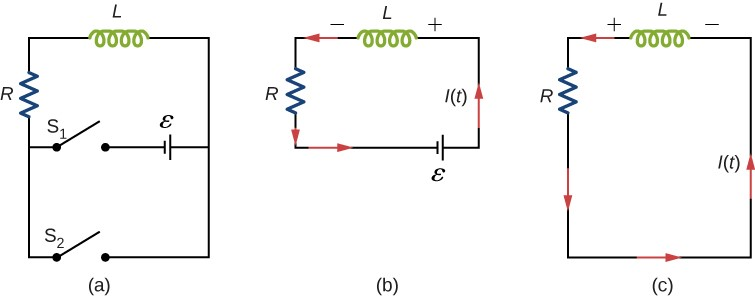
\includegraphics[width=0.5\textwidth]{figures/rl.jpeg}
\caption{\label{fig:rl} A circuit diagram of a DC emf with a resistor, inductor, and two switches.}
\end{figure}

\begin{enumerate}
\item Consider Fig. \ref{fig:rl}.  There is a battery connected to a resistor $R$ and and inductor $L$ via switch 1.  Switch 2 connects $L$ and $R$.  In algebraic terms, what are the currents when: (a) $t=0$, when switch 1 is closed, and (b) when $t\gg\tau$? \\ \vspace{2.0cm}
\item (a) What is $\tau$ when $R = 1$ k$\Omega$, and $L = 0.2$ Henries? (b) What will the time constant $\tau$ be if we double $R$ and quadruple $L$? \\ \vspace{0.5cm}
\item If switch 1 is open and switch 2 closed after $t\gg\tau$, what time passes before the current is reduced to half of its original value? \\ \vspace{1cm}
\end{enumerate}

\section{Reactance and Impedance}

\begin{enumerate}
\item (a) What is the reactance, in ohms, of a $2.5$ $\mu$F capacitor at 1.4 kHz? (b) What is the reactance of a $5.0$ mH inductor at this same frequency? (c) Now add (in series) a $1$ k$\Omega$ resistor.  What is the total impedance at at this frequency? (d) What is the resonance frequency? (e) What is the total impedance at 1.4 MHz? \\ \vspace{3.5cm}
\item For an RLC series circuit having a 40.0 $\Omega$ resistance, a 3.00 mH inductance, a 5.00 $\mu$F capacitance, and a voltage source with a $V_{\rm rms}$ of 120 V: (a) calculate the \textit{phase angle}, $\phi$, and \textit{power factor}, $\cos\phi$, for $f = 60$ Hz. (b) What is the average power at 60.0 Hz? (c) Find the average power at the resonance frequency.
\end{enumerate}
\end{document}
